The study of programming language theory can be understood in part as the study of \textbf{inference systems}.\footnote{
  In some settings, these are called \textbf{formal systems} or \textbf{deductive systems}, though it's my sense that there's no real consensus as to what exactly these terms mean.
}
A programming language\textemdash in the sense of the techology that we use when we program\textemdash is just an \textit{implementation} of a collection of inference systems.

We begin with a picture.
As we said in \Cref{ch:intro}, when we program we type a bunch of characters into a file.
Of the sequence of characters we can type, only a handful of them are valid \textit{sequences of tokens} in our programming language.
For example, \codel{let} is a keyword of OCaml, \codel{1.223} is a floating point literal, \codel{\%} is an operator, and \codel{yasn3\_\_} is a valid variable name.
These are all valid tokens in OCaml.\footnote{We'll take of the question of what makes a valid token more formally in \ref{}.}
Furthermore, OCaml requires that tokens are separated by whitespace, so any whitespace-separated combination of these is a valid sequence of tokens.
But \codel{,,A,,} is a meaningless sequences of symbols from OCaml's perspective, and cannot appear in a valid sequence of tokens.

Now, of the possible sequences of tokens, only a handful of those constitute \textit{well-formed programs}.
For example, \codel{let f x = x + 2} is a valid OCaml program, whereas \codel{let f rec = =} is not, though both are valid sequences of tokens.

Of the well-formed programs, only a handful make sense as programs; said another way, only a handful are \textit{well-typed programs}.
For example, \codel{let rec f x = f x} is well-typed, whereas \codel{let rec f x = f + x} is not, though both are well-formed programs.
And of the well-typed programs, only a handful of \textit{those} make sense as computations; said another way, only a handful can be successfully \textit{evaluated}.

The above observations can be visualized as nested sets (\Cref{fig:nested-progs}).
Note that things get interesting in the relationship between well-typed programs and programs that have values.
We'll take this up in-depth when we cover type systems in \Cref{ch:type-systems}.

\begin{figure}
  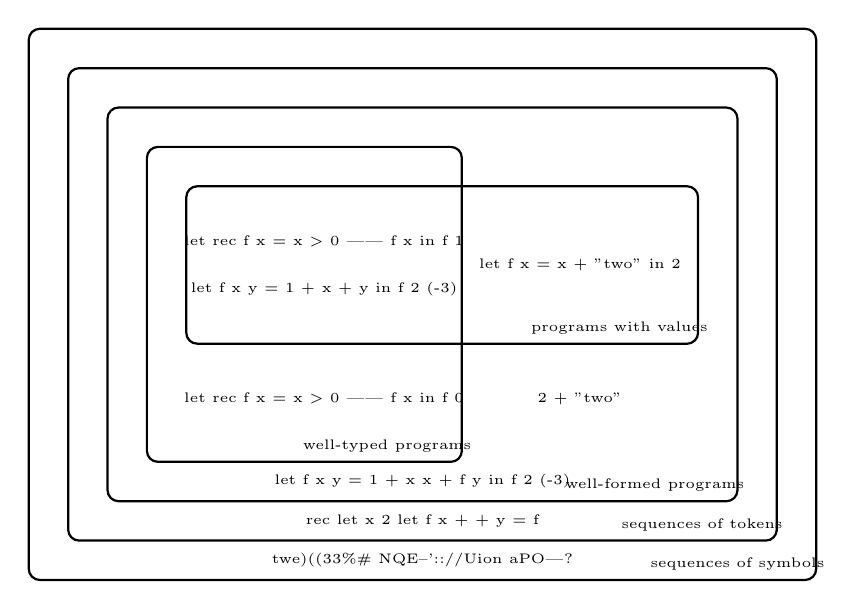
\begin{tikzpicture}
    \draw[thick, rounded corners] (0,0) rectangle (10, 7);
    \node at (9.0,0.2) {\tiny sequences of symbols};
    \node at (5.0,0.25) {\tiny \codel{twe)((33\%\@\#  NQE--':://Uion  aPO^^<?}};
    \draw[thick, rounded corners] (0.5, 0.5) rectangle (9.5, 6.5);
    \node at (8.55,0.7) {\tiny sequences of tokens};
    \node at (5.0,0.75) {\tiny \codel{rec let x 2 let f x + + y = f}};
    \draw[thick, rounded corners] (1, 1) rectangle (9, 6);
    \node at (7.95,1.2) {\tiny well-formed programs};
    \node at (5.0,1.25) {\tiny \codel{let f x y = 1 + x x + f y in f 2 (-3)}};
    \draw[thick, rounded corners] (1.5, 1.5) rectangle (5.5, 5.5);
    \node at (4.55,1.7) {\tiny well-typed programs};
    \node  at (3.75,2.3) {\tiny \codel{let rec f x = x > 0 || f x in f 0}};
    \node at (3.75,3.7) {\tiny \codel{let f x y = 1 + x + y in f 2 (-3)}};
    \node  at (3.75,4.3) {\tiny \codel{let rec f x = x > 0 || f x in f 1}};
    \draw[thick, rounded corners] (2, 3) rectangle (8.5, 5);
    \node  at (7.0,4.0) {\tiny \codel{let f x = x + "two" in 2}};
    \node  at (7.0,2.3) {\tiny \codel{2 + "two"}};
    \node at (7.5,3.2) {\tiny programs with values};
  \end{tikzpicture}
  \centering
  \caption{
    Visualization of nested classes of programs.
    In order to make the graphic simpler, the code examples are actually OCaml \textit{expressions}, not programs.
  }
  \label{fig:nested-progs}
\end{figure}
%
Our goal is to transform a sequence of characters representing a program into the output \textit{value} of the program.
This is done by successive transformations, each of which corresponds roughly to one of these nested sets:
\begin{itemize}
\item determining valid sequences of tokens in part of \textit{lexical analysis};
\item determining well-formed programs is part of \textit{parsing} or \textit{syntactic analysis};
\item determining well-typed programs is part of \textit{type-checking} or \textit{static semantic analysis};
\item determining the value of a program is part of \textit{evaluation} or \textit{dynamic semantic analysis}.
\end{itemize}
And each transformation has a corresponding inference system that \textit{formally} describes which inputs are \enquote{good} and which are \enquote{junk}.

\bigskip

\noindent In this chapter we will:
\begin{itemize}
\item formally define \textbf{inference rules}, i.e, the rules which govern when we can derive new judgments from judgements we've already derived in an inference system;
\item use \textbf{derivations} to demonstrate that a judgment is derivable in an inference system;
\item present an extended example which consists of a collection of inference systems that define the syntax, typing behavior, and evaluation behavior of a simple programming language for a calculator.
\end{itemize}

\section{Inference Rules}

An \textbf{inference system} is determined by a collection of \textbf{inference rules}.
These inference rules describe what new information we're allowed to \textit{infer} given previously inferred information.
Inference rules will generally have the following form.
\begin{mathpar}
  \inferrule*[right=addTwo]{
    m$ is even$
    \and
    $\hl{$n = m + 2$}$
  }{
    n$ is even$
  }
\end{mathpar}
This inference rule expresses that we can infer a number $n$ is even if we already know that $n = m + 2$ and $m$ is even (i.e., if $n - 2$ is even).
We begin by looking at the general anatomy of inference rules.

An inference system is defined over a fixed class of \textbf{judgments}.
We think of judgments as the things we can say while inferring something.
Mathematically speaking, judgments can be anything we want, i.e., elements of an arbitrary set.
Practically speaking, we'll always take judgments to be \textit{statements} parametrized by some other set.
\begin{example}
  \label{ex:evens-odds}
  If we're interested in the parity of natural numbers, we may take our set of judgments $\mathcal J$ to be all statements of the form
  \begin{align*}
    \text{$n$ is even} \qquad \text{or} \qquad \text{$n$ is odd}
  \end{align*}
  So \enquote{$7$ is even} and \enquote{$111$ is odd} are both judgments in $\mathcal J$.
  Note that statements in $\mathcal J$ are parametrized by the set of natural numbers.
\end{example}
We'll call something like \enquote{$n$ is even} a \textbf{parameterized judgment} and something like \enquote{$4$ is even} a \textbf{concrete judgment}, or just a judgment if it's clear from context that it's concrete.
In particular, we'll say \enquote{$110$ is odd} is an \textbf{instance} of the parameterized judgment \enquote{$n$ is odd.}

\begin{remark}
We'll be a bit cavalier about the distinction between parametrized and concrete judgments.
For example, we'll say that concrete judgments are also parameterized judgments, insofar as they're parametrized by no parameters.
Likewise, we'll say that a parameterized judgment is in a set $\mathcal J$ when we really mean that its instances are in $\mathcal J$.
\end{remark}
An \textbf{inference rule} is a way of describing what judgments we're allowed to infer given we've already inferred some other judgments.
They also often include additional statements that need to hold in order for a given rule to be applied; these are called \textbf{side conditions}.\footnote{
In what follows we \hl{highlight} side conditions to make clear that they are not formal judgments.
}
The following is the general definition of an inference rule.
It's important that we understand this definition, but not on our first pass; make sure to lean on the intuitions we've been trying to develop here as you work through this chapter, and come back to this definition potentially several times.
\begin{definition}
  An \textbf{inference rule} named \textsc{ruleName} is a nonempty sequence of parameterized judgments $J_1, \dots J_k, J_{k + 1}$ along with a collection of statements $S_1, \dots, S_l$ depending on the parameters used in those judgments. An inference rule is denoted by
  \begin{mathpar}
    \inferrule*[right=ruleName]{
      J_1 \quad \dots \quad J_k
      \and
      $\hl{$S_1$}$ \quad \dots \quad $\hl{$S_l$}$
    }{
      J_{k + 1}
    }
  \end{mathpar}
  We say that a concrete judgment $J_{k + 1}'$ \textbf{follows from} the concrete judgments $J_1', \dots, J_k'$ (by \textsc{ruleName}) if $J_i'$ is an instance of $J_i$ for each index $i$ and all statements $S_1, \dots, S_l$ hold for the parameters used in the given judgments.
  We'll often also denote this by
  \begin{mathpar}
    \inferrule*[right=ruleName]{
      J_1' \quad \dots \quad J_k'
    }{
      J_{k + 1}'
    }
  \end{mathpar}
  and say that this is an \textbf{instance} of the rule \textsc{ruleName}.
  We'll also call this an \textbf{inference}.
\end{definition}
We call the judgments above the line \textbf{antecedences} and the judgment below called the \textbf{consequent}.
An inference rule may have no side-condition or no antecedents.
An inference rule with no antecedents is called an \textbf{axiom}.

\begin{example}
  The inference
  \begin{mathpar}
    \inferrule*[right=addTwo]{
      10$ is even$
    }{
      12$ is even$
    }
  \end{mathpar}
  is an instance of the rule \textsc{addTwo} above.
  In particular, the side condition \hl{$12 = 10 + 2$} holds.
  Note that the side condition is not included in the instance, it's checked \enquote{offline}.
  Also note that
  \begin{mathpar}
    \inferrule*[right=addTwo]{
      11$ is even$
    }{
      13$ is even$
    }
  \end{mathpar}
  is an instance of \textsc{addTwo}.
  It expresses that, hypothetically, if $11$ were even then $13$ would be even.
\end{example}

\section{Derivations}

At this point, we can give a basic definition of an inference system.

\begin{definition}
  An \textbf{inference system} over a set of judgment $\mathcal J$ is a collection of inference rules over $\mathcal J$.
\end{definition}

\begin{example}
  \label{ex:even-system}
  Let $\mathcal J$ be as in \Cref{ex:evens-odds}.
  We can consider the inference system given by the following two inference rules (note that these rules do not say anything about odd numbers).
  \begin{mathpar}
    \inferrule*[right=zero]{
    }{
      0$ is even$
    }
    \and
    \inferrule*[right=addTwo]{
      m$ is even$
      \and
      $\hl{$n = m + 2$}$
    }{
      n$ is even$
    }
  \end{mathpar}
\end{example}
%
What we're interested in with regard to inference systems is the collection of judgments that are \textit{possible} to infer.
We make this concrete with the notion of a \textbf{derivation}, which is used to demonstrate that it's possible to infer a given judgment in an inference system by invocations of its inference rules (see \Cref{ch:trees} for a refresher on trees).

\begin{definition}
  A \textbf{derivation} of the judgment $J$ in an inference system $\mathcal I$ is a tree $T$ with the following properties:
  \begin{itemize}
  \item The values of $T$ are judgments from $\mathcal J$;
  \item $\troot{T}$ is $J$;
  \item For every node of $T$ of the form $\tnode(K, T_1, \dots, T_l)$
    \begin{mathpar}
      \inferrule*[right=rule]{
        \troot{T_1}
        \and
        \dots
        \and
        \troot{T_l}
      }{
        K
      }
    \end{mathpar}
    is an instance of \textsc{rule}, where \textsc{rule} appears in $\mathcal I$.
  \end{itemize}
\end{definition}
%
In particular, the leaves of $T$ are instances of axioms in $\mathcal I$.
It's in this definition that we see why axioms are important: without them, our derivations can't start anywhere.
\Cref{fig:8-is-even} has a derivation of the judgment \enquote{$8$ is even} in the inference system from \Cref{ex:even-system}.
It's not a terribly interesting derivation, but it captures the form of reasoning we're allowed to do in this system: $8$ is even because $6$ is even, which holds because $4$ is even, which holds because $2$ is even, which holds because $0$ is even, which holds by fiat.
\begin{remark}
  Even though derivations are trees, we present them bottom-up as stacks of inferences.
  This is, in part, because it captures the structure of a derivation more naturally, but it's also historical: Gerhard Gentzen established much of the notation we use here (and in the mathematical field called \textit{proof theory}) in the 1930s \cite{gentzen1964investigations}.
\end{remark}
%

\begin{example}
  \label{ex:even-alt}
  Let's consider a slightly more interesting inference system.
  We can define an alternative system for parity reasoning which takes advantage of what we know about odd numbers.
  \begin{mathpar}
    \inferrule*[right=zero]{
    }{
      0$ is even$
    }
    \and
    \inferrule*[right=one]{
    }{
      1$ is odd$
    }
    \and
    \inferrule*[right=odd]{
      m$ is even$
      \and
      $\hl{$n = m + 1$}$
    }{
      n$ is odd$
    }
    \and
    \inferrule*[right=even]{
      m$ is odd$
      \and
      n$ is odd$
      \and
      $\hl{$k = m + n$}$
    }{
      k$ is even$
    }
  \end{mathpar}
\end{example}
\Cref{fig:8-is-even-again} is a derivation of \enquote{8 is even} is this alternative system.
The primary takeaway: different inference systems provide us with different forms of reasoning.
In this alternative system, we have to first separate $8$ into two summands and reason about them separately.
This system also differs from the one in \Cref{ex:even-system} because a judgment may have multiple proofs.

\begin{exercise}
  Give another derivation of \enquote{$8$ is even} in this system from \Cref{ex:even-alt}.
\end{exercise}

\begin{exercise}
  \textbf{(Challenge)}
  Prove that \enquote{$n$ is even} is derivable in the system from \Cref{ex:even-system} if and only if it's derivable in the system from \Cref{ex:even-alt}.
\end{exercise}

\begin{figure}
  \begin{prooftree}
    \AxiomC{}
    \RightLabel{\textsc{zero}}
    \UnaryInfC{$0$ is even}
    \RightLabel{\textsc{addTwo}}
    \UnaryInfC{$2$ is even}
    \RightLabel{\textsc{addTwo}}
    \UnaryInfC{$4$ is even}
    \RightLabel{\textsc{addTwo}}
    \UnaryInfC{$6$ is even}
    \RightLabel{\textsc{addTwo}}
    \UnaryInfC{$8$ is even}
  \end{prooftree}
  \caption{A derivation of \enquote{$8$ is even} in the inference system from \Cref{ex:even-system}}
  \label{fig:8-is-even}
\end{figure}

\begin{figure}
  \begin{prooftree}
    \AxiomC{}
    \RightLabel{\small \textsc{one}}
    \UnaryInfC{$1$ is odd}
    \AxiomC{}
    \RightLabel{\small \textsc{one}}
    \UnaryInfC{$1$ is odd}
    \RightLabel{\small \textsc{even}}
    \BinaryInfC{$2$ is even}
    \RightLabel{\small \textsc{odd}}
    \UnaryInfC{$3$ is odd}
    \AxiomC{}
    \RightLabel{\small \textsc{one}}
    \UnaryInfC{$1$ is odd}
    \RightLabel{\small \textsc{even}}
    \BinaryInfC{$4$ is even}
    \RightLabel{\small \textsc{odd}}
    \UnaryInfC{$5$ is odd}
    \AxiomC{}
    \RightLabel{\small \textsc{one}}
    \UnaryInfC{$1$ is odd}
    \AxiomC{}
    \RightLabel{\small \textsc{one}}
    \UnaryInfC{$1$ is odd}
    \RightLabel{\small \textsc{even}}
    \BinaryInfC{$2$ is even}
    \RightLabel{\small \textsc{odd}}
    \UnaryInfC{$3$ is odd}
    \RightLabel{\small \textsc{even}}
    \BinaryInfC{$8$ is even}
  \end{prooftree}
  \caption{Derivation of \enquote{$8$ is even} in the inference system from \Cref{ex:even-alt}}
  \label{fig:8-is-even-again}
\end{figure}

\section{Extended Example: Calculator}

\begin{figure}
\begin{align*}
\bnfnt{expr} &\bnfeq \bnft( \ \bnft+ \ \bnfnt{expr} \ \bnfnt{expr} \ \bnft) \\
&\bnfaltn \bnft( \ \bnft* \ \bnfnt{expr} \ \bnfnt{expr} \ \bnft) \\
&\bnfaltn \bnft( \ \bnft= \ \bnfnt{expr} \ \bnfnt{expr} \ \bnft) \\
&\bnfaltn \bnft( \ \bnft? \ \bnfnt{expr} \ \bnfnt{expr} \ \bnfnt{expr} \ \bnft) \\
&\bnfaltn \bnft 0 \bnfalt \bnft 1
\end{align*}
\caption{Lisp-like syntax for a simple calculator}
\label{fig:calc-syntax}
\end{figure}

We now consider several inference systems defined over judgments about expressions for a calculator with lisp-like syntax.
This syntax will only allow for 8 possible tokens: \codel{(}, \codel{)}, \codel{+}, \codel{*}, \codel{=}, \codel{?}, \codel{0}, and \codel{1}.
Anticipating the next chapter, the formal grammar for such expressions is give in \Cref{fig:calc-syntax}.
You're not expected to understand this specification; it's just meant to give a hint of what is to come.

We begin by defining an inference system that determines which sequences of tokens constitute well-formed expressions (\Cref{fig:wf-sys}).\footnote{The astute reader might notice that we're skipping lexical analysis. This is partly for simplicity, but it's also because all our tokens are exactly one character long, and so, barring issues of whitespace for now, \textit{any} sequence of valid characters constitutes a valid sequence of tokens.}
This system is defined over judgments of the form \enquote{$e \in \mathsf{WF}$} where $e$ is a sequence of tokens.
It captures in its inference rules that operators appear before their arguments, and that all invocations of an operator are surrounded in parentheses, e.g.,
\begin{align*}
  \codel{( * ( + 1 1 ) ( + 1 1 ) )}
\end{align*}
is a well-formed expression, and we can derive this judgment formally (\Cref{fig:wf-deriv}).
Let’s take a brief moment to read what each of these rules says.
\begin{itemize}
\item \textsc{zeroS} says that $\codel 0$ is a well-formed expression, no matter what.
\item \textsc{oneS} says that $\codel 1$ is a well-formed expression, no matter what.
\item \textsc{addS} says that that if $e_1$ and $e_2$ are well-formed expressions, then so is $\codel( \ \codel+ \ e_1 \ e_2 \ \codel)$.
\item \textsc{mulS} says that that if $e_1$ and $e_2$ are well-formed expressions, then so is $\codel( \ \codel* \ e_1 \ e_2 \ \codel)$.
\item \textsc{eqS} says that that if $e_1$ and $e_2$ are well-formed expressions, then so is $\codel( \ \codel= \ e_1 \ e_2 \ \codel)$.
\item \textsc{condS} says that that if $e_1$, $e_2$, and $e_3$ are well-formed expressions, then so is $\codel( \ \codel ? \ e_1 \ e_2 \ e_3 \ \codel)$.
\end{itemize}
We cannot stress this enough: \textit{inference rules are formal shorthand for expressing rules which can also be expressed in natural language.}
The natural language descriptions above may at first seem a lot easier to read.
But over time, as you learn to read inference rules, you'll find that they are \textit{much} more convenient, especially when the inference system has $50$ (or even $500$) rules.
\begin{exercise}
  Show that $\codel{( = ( = 0 0 ) 1 )} \in \mathsf{WF}$ by deriving it in the inference system from \Cref{fig:wf-sys}.
\end{exercise}

\begin{figure}
  \begin{mathpar}
    \inferrule*[right=zeroS]{
    }{
      \codel 0 \in \mathsf{WF}
    }
    \and
    \inferrule*[right=oneS]{
    }{
      \codel 1 \in \mathsf{WF}
    }
    \and
    \inferrule*[right=addS]{
      e_1 \in \mathsf{WF}
      \and
      e_2 \in \mathsf{WF}
    }{
      \codel( \ \codel+ \ e_1 \ e_2 \ \codel) \in \mathsf{WF}
    }
    \and
    \inferrule*[right=mulS]{
      e_1 \in \mathsf{WF}
      \and
      e_2 \in \mathsf{WF}
    }{
      \codel( \ \codel* \ e_1 \ e_2 \ \codel) \in \mathsf{WF}
    }
    \and
    \inferrule*[right=eqS]{
      e_1 \in \mathsf{WF}
      \and
      e_2 \in \mathsf{WF}
    }{
      \codel( \ \codel= \ e_1 \ e_2 \ \codel) \in \mathsf{WF}
    }
    \and
    \inferrule*[right=condS]{
      e_1 \in \mathsf{WF}
      \and
      e_2 \in \mathsf{WF}
      \and
      e_3 \in \mathsf{WF}
    }{
      \codel( \ \codel? \ e_1 \ e_2 \ e_3 \ \codel) \in \mathsf{WF}
    }
    \and
  \end{mathpar}
  \caption{Inference systems for well-formed expressions in the language from \Cref{fig:calc-syntax}}
  \label{fig:wf-sys}
\end{figure}

\begin{figure}
  \begin{prooftree}
    \AxiomC{}
    \RightLabel{\small \textsc{oneS}}
    \UnaryInfC{$\codel 1 \in \mathsf{WF}$}
    \AxiomC{}
    \RightLabel{\small \textsc{oneS}}
    \UnaryInfC{$\codel 1 \in \mathsf{WF}$}
    \RightLabel{\small \textsc{addS}}
    \BinaryInfC{$\codel{( + 1 1 )} \in \mathsf{WF}$}
    \AxiomC{}
    \RightLabel{\small \textsc{oneS}}
    \UnaryInfC{$\codel 1 \in \mathsf{WF}$}
    \AxiomC{}
    \RightLabel{\small \textsc{oneS}}
    \UnaryInfC{$\codel 1 \in \mathsf{WF}$}
    \RightLabel{\small \textsc{addS}}
    \BinaryInfC{$\codel{( + 1 1 )} \in \mathsf{WF}$}
    \RightLabel{\small \textsc{mulS}}
    \BinaryInfC{$\codel{( * ( + 1 1 ) ( + 1 1 ) )} \in \mathsf{WF}$}
  \end{prooftree}
  \caption{Derivation of \enquote{$\codel{( * ( + 1 1 ) ( + 1 1 ) )} \in \mathsf{WF}$} in the system from \Cref{fig:wf-sys}.}
  \label{fig:wf-deriv}
\end{figure}

\begin{remark}
  Keep in mind that these expressions don't \textit{mean} anything yet, even though we can guess that \enquote{\codel+} will stand for addition and \enquote{\codel{*}} will stand for multiplication.
  The expression
  \begin{align*}
    \codel{( + ( = 1 1 ) ( = 0 1 ) )}
  \end{align*}
  is also a well-formed expression, even though this may not make sense if we interpret \enquote{\codel{=}} as an equality operator which evalutes to a Boolean value.
\end{remark}
%
Once we've defined the well-formed expressions using an inference system, we can prove things about well-formed expressions using induction on derivations (see \Cref{ch:trees}).
\begin{exercise}
  Prove using induction on derivations that if $e \in \mathsf{WF}$, then there are the same number of left parentheses as right parentheses in $e$.
\end{exercise}
%
In addition to proving things via structural induction, we can also define properties on well-formed expressions by defining new inference systems.
In particular, we can use the notion of a well-formed expression in other inference systems.

Suppose, for example, we want to reason about how many symbols are in a given well-formed expression.
We can define an inference system to do this sort of reasoning (\Cref{fig:sym-sys}).
This system is defined over judgments of the form \enquote{\#($e$) = $n$} where $e$ ranges over well-formed expressions (i.e., we can derive \enquote{$e \in \mathsf{WF}$} in the previously defined inference system) and $n$ ranges over natural numbers.
The rules in this system express that \codel0 and \codel1 have $1$ symbol, and every other expression has 3 plus [the number of symbols in its subexpressions] many symbols.
We can formally derive that the expression
\begin{align*}
  \codel{( * ( + 1 1 ) ( + 1 1 ) )}
\end{align*}
has $13$ symbols (\Cref{fig:sym-deriv}).

\begin{figure}
  \begin{mathpar}
    \inferrule*[right=zeroC]{
    }{
      \#(\codel 0) = 1
    }
    \and
    \inferrule*[right=oneC]{
    }{
      \#(\codel 1) = 1
    }
    \and
    \inferrule*[right=addC]{
      \#(e_1) = m
      \and
      \#(e_2) = n
      \and
      $\hl{$k = m + n + 3$}$
    }{
      \#(\codel( \ \codel+ \ e_1 \ e_2 \ \codel)) = k
    }
    \and
    \inferrule*[right=mulC]{
      \#(e_1) = m
      \and
      \#(e_2) = n
      \and
      $\hl{$k = m + n + 3$}$
    }{
      \#(\codel( \ \codel* \ e_1 \ e_2 \ \codel)) = k
    }
    \and
    \inferrule*[right=eqC]{
      \#(e_1) = m
      \and
      \#(e_2) = n
      \and
      $\hl{$k = m + n + 3$}$
    }{
      \#(\codel( \ \codel= \ e_1 \ e_2 \ \codel)) = k
    }
    \and
    \inferrule*[right=condC]{
      \#(e_1) = l
      \and
      \#(e_2) = m
      \and
      \#(e_3) = n
      \and
      $\hl{$k = l + m + n + 3$}$
    }{
      \#(\codel( \ \codel? \ e_1 \ e_2 \ e_3 \ \codel)) = k
    }
  \end{mathpar}
  \caption{Inference system for determining the number of symbols in a well-formed expression}
  \label{fig:sym-sys}
\end{figure}

\begin{figure}
  \begin{prooftree}
    \AxiomC{}
    \RightLabel{\small \textsc{oneC}}
    \UnaryInfC{$\#(\codel{1}) = 1$}
    \AxiomC{}
    \RightLabel{\small \textsc{oneC}}
    \UnaryInfC{$\#(\codel{1}) = 1$}
    \RightLabel{\small \textsc{addC}}
    \BinaryInfC{$\#(\codel{( + 1 1 )}) = 5$}
    \AxiomC{}
    \RightLabel{\small \textsc{oneC}}
    \UnaryInfC{$\#(\codel{1}) = 1$}
    \AxiomC{}
    \RightLabel{\small \textsc{oneC}}
    \UnaryInfC{$\#(\codel{1}) = 1$}
    \RightLabel{\small \textsc{addC}}
    \BinaryInfC{$\#(\codel{( + 1 1 )}) = 5$}
    \RightLabel{\small \textsc{mulC}}
    \BinaryInfC{$\#(\codel{( * ( + 1 1 ) ( + 1 1 ) )}) = 13$}
  \end{prooftree}
  \caption{Derivation of \enquote{$\#(\codel{( * ( + 1 1 ) ( + 1 1 ) )}) = 13$} in the system from \Cref{fig:sym-sys}}
  \label{fig:sym-deriv}
\end{figure}

\begin{exercise}
  Show that $\#(\codel{( = ( = 0 0 ) 1 )}) = 9$ by deriving of it in the inference system from \Cref{fig:sym-sys}.
\end{exercise}

We'd like to now start thinking about the \textit{meaning} of these expressions.
First, we have to contend with the fact that not all well-formed expressions are meaningful.
The expression
  \codel{( = ( = 0 0 ) 1 )}
cannot be evaluated successfully because it would require us to compare two values that aren't the \enquote{same kind of thing}.
Formally, the \enquote{kind of thing} a value can be is called its \textbf{type}.
There are two types of values that an expression can evaluate to in our calculator language: a number (\codel{int}) or a Boolean value (\codel{bool}).

\begin{remark}
  It would be possible to represent Boolean values as numbers; this is done, for example, in C.
  Then there would be a single type of value in our lanugage.
  We'll avoid doing this, in part because it makes our example less interesting, but also because there are some serious problems that arise when we design programming languages this way.
\end{remark}
%
We can define an inference system which determines the type of an expression, if it has one.
This means that the system has two purposes: (1) it delineates a set of expressions that have values (i.e., which we can evaluate), and (2) it determines the type of that value \textit{before} we've evaluated the expression (\Cref{fig:calc-ty-sys}).

\begin{figure}
  \begin{mathpar}
    \inferrule*[right=zeroT]{
    }{
      \codel0 : \codel{int}
    }
    \and
    \inferrule*[right=oneT]{
    }{
      \codel1 : \codel{int}
    }
    \and
    \inferrule*[right=addT]{
      e_1 : \codel{int}
      \and
      e_2 : \codel{int}
    }{
      \codel( \ \codel+ \ e_1 \ e_2 \ \codel) : \codel{int}
    }
    \and
    \inferrule*[right=mulT]{
      e_1 : \codel{int}
      \and
      e_2 : \codel{int}
    }{
      \codel( \ \codel* \ e_1 \ e_2 \ \codel) : \codel{int}
    }
    \and
    \inferrule*[right=eqT]{
      e_1 : t_1
      \and
      e_2 : t_2
      \and
      $\hl{$t_1 = t_2$}$
    }{
      \codel( \ \codel= \ e_1 \ e_2 \ \codel) : \codel{bool}
    }
    \and
    \inferrule*[right=condT]{
      e_1 : \codel{bool}
      \and
      e_2 : t_2
      \and
      e_3 : t_3
      \and
      $\hl{$t_2 = t_3$}$
    }{
      \codel( \ \codel? \ e_1 \ e_2 \ e_3 \ \codel) : t_2
    }
  \end{mathpar}
  \caption{Inference system for determining the type of an expression}
  \label{fig:calc-ty-sys}
\end{figure}

This system is defined over judgments of the form \enquote{$e : t$} where $e$ is a well-formed expression and $t$ is either \codel{int} or \codel{bool}.
We read a judgment of this form as \enquote{$e$ is of type $t$} or \enquote{$e$ is a $t$}.
Let's again take a brief moment to read what each of these rules says.
\begin{itemize}
\item \textsc{zeroT} says \codel 0 is a \codel{int}, no matter what.
\item \textsc{oneT} says \codel 1 is a \codel{int}, no matter what.
\item \textsc{addT} says if $e_1$ is a \codel{int} (i.e., evaluates to a number) and $e_2$ is a \codel{int}, then $\codel( \ \codel+ \ e_1 \ e_2 \ \codel)$ is a \codel{int}.
  In particular, we can only add numbers, not Boolean values.
\item \textsc{mulT} says if $e_1$ is a \codel{int} (i.e., evaluates to a number) and $e_2$ is a \codel{int}, then $\codel( \ \codel* \ e_1 \ e_2 \ \codel)$ is a \codel{int}.
  In particular, we can only multiply numbers, not Boolean values.
\item \textsc{eqT} says if $e_1$ and $e_2$ are the same type then we can compare them, and $\codel( \ \codel= \ e_1 \ e_2 \ \codel)$ is a \codel{bool}. In particular, we can't compare a number with a Boolean value.
\item \textsc{condT} says if $e_1$ is a \codel{bool}, and $e_2$ and $e_3$ are the same type, then we can condition on the value of $e_1$ to get either the value of $e_2$ or $e_3$, and the type of $\codel( \ \codel? \ e_1 \ e_2 \ e_3 \ \codel)$ is the same as that of $e_2$ and $e_3$.
\end{itemize}
See \Cref{fig:calc-ty-deriv} for an example derivation in this system.
\begin{exercise}
  Show that $\codel{( = ( + 0 0 ) 1 )} : \codel{bool}$ by deriving it in the inference system from \Cref{fig:calc-ty-sys}.
\end{exercise}
\begin{figure}
  \begin{prooftree}
    \AxiomC{}
    \RightLabel{\small \textsc{oneT}}
    \UnaryInfC{$\codel{1} : \codel{int}$}
    \AxiomC{}
    \RightLabel{\small \textsc{oneT}}
    \UnaryInfC{$\codel{1} : \codel{int}$}
    \RightLabel{\small \textsc{eqT}}
    \BinaryInfC{$\codel{( = 1 1 )} : \codel{bool}$}
    \AxiomC{}
    \RightLabel{\small \textsc{oneT}}
    \UnaryInfC{$\codel{1} : \codel{int}$}
    \AxiomC{}
    \RightLabel{\small \textsc{oneT}}
    \UnaryInfC{$\codel{1} : \codel{int}$}
    \RightLabel{\small \textsc{addT}}
    \BinaryInfC{$\codel{( + 1 1 )} : \codel{int}$}
    \AxiomC{}
    \RightLabel{\small \textsc{oneT}}
    \UnaryInfC{$\codel{1} : \codel{int}$}
    \AxiomC{}
    \RightLabel{\small \textsc{zeroT}}
    \UnaryInfC{$\codel{0} : \codel{int}$}
    \RightLabel{\small \textsc{mulT}}
    \BinaryInfC{$\codel{( * 1 0 )} : \codel{int}$}
    \RightLabel{\small \textsc{condT}}
    \TrinaryInfC{$\codel{( ? ( = 1 1 ) ( + 1 1 ) ( * 1 0 ) )} : \codel{int}$}
  \end{prooftree}
  \caption{Derivation of \enquote{$\codel{( ? ( = 1 1) ( + 1 1 ) ( * 1 0 ) )} : \codel{int}$} in the system from \Cref{fig:calc-ty-sys}}
  \label{fig:calc-ty-deriv}
\end{figure}
Finally, we can define an inference system for determining the value of an expression in our language (\Cref{fig:calc-eval-sys}).
This system is defined over judgments of the form \enquote{$e \Downarrow v$}, which we read as \enquote{$e$ evaluates to $v$} where $e$ ranges over well-formed expressions, and $v$ ranges over numbers ($\mathbb N$) or Boolean values ($\{\mathsf{true}, \mathsf{false}\}$).
Let's on last time take a moment to read what each of these rules says.
\begin{itemize}
\item \textsc{zeroE} says \codel0 evaluates to the number $0$.
\item \textsc{oneE} says \codel1 evaluates to the number $1$.
\item \textsc{addE} says if $e_1$ evaluates to $m$ and $e_2$ evaluates to $n$, then $\codel( \ \codel+ \ e_1 \ e_2 \ \codel)$ evaluates to $m + n$.
\item \textsc{mulE} says if $e_1$ evaluates to $m$ and $e_2$ evaluates to $n$, then $\codel( \ \codel* \ e_1 \ e_2 \ \codel)$ evaluates to $m \times n$.
\item \textsc{eqTrueE} says if $e_1$ evaluates to $v_1$ and $e_2$ evaluates to $v_2$, and $v_1$ and $v_2$ are the same then $\codel( \ \codel= \ e_1 \ e_2 \ \codel)$ evaluates to $\mathsf{true}$.
\item \textsc{eqFalseE} says if $e_1$ evaluates to $v_1$ and $e_2$ evaluates to $v_2$, and $v_1$ and $v_2$ are \textit{not} the same then $\codel( \ \codel= \ e_1 \ e_2 \ \codel)$ evaluates to $\mathsf{false}$.
\item \textsc{ifTrueE} says if $e_1$ evaluates to $\mathsf{true}$ and $e_2$ evaluates to $v$, then $\codel( \ \codel? \ e_1 \ e_2 \ e_3 \ \codel)$ evaluates to $v$.
  In particular, $e_3$ does not need to be evaluated.
\item \textsc{ifFalseE} says if $e_1$ evaluates to $\mathsf{true}$ and $e_3$ evaluates to $v$, then $\codel( \ \codel? \ e_1 \ e_2 \ e_3 \ \codel)$ evaluates to $v$.
  In particular, $e_2$ does not need to be evaluated.
\end{itemize}
See \Cref{fig:calc-eval-deriv} for an example derivation in this system.
Notice that the side conditions are where the \enquote{real} computation happens, e.g., the (add) rule draws a correspondence between the \codel{+} operator in our language and normal addition \enquote{$+$} in the side condition.

\begin{figure}
  \begin{mathpar}
    \inferrule*[right=zeroE]{
    }{
      \codel0 \Downarrow 0
    }
    \and
    \inferrule*[right=oneE]{
    }{
      \codel1 \Downarrow 1
    }
    \and
    \inferrule*[right=addE]{
      e_1 \Downarrow v_1
      \and
      e_2 \Downarrow v_2
      \and
      $\hl{$v = v_1 + v_2$}$
    }{
      \codel( \ \codel+ \ e_1 \ e_2 \ \codel) \Downarrow v
    }
    \and
    \inferrule*[right=mulE]{
      e_1 \Downarrow v_1
      \and
      e_2 \Downarrow v_2
      \and
      $\hl{$v = v_1 \times v_2$}$
    }{
      \codel( \ \codel* \ e_1 \ e_2 \ \codel) \Downarrow v
    }
    \and
    \inferrule*[right=eqTrue]{
      e_1 \Downarrow v_1
      \and
      e_2 \Downarrow v_2
      \and
      $\hl{$v_1 = v_2$}$
    }{
      \codel( \ \codel= \ e_1 \ e_2 \ \codel) \Downarrow \mathsf{true}
    }
    \and
    \inferrule*[right=eqFalse]{
      e_1 \Downarrow v_1
      \and
      e_2 \Downarrow v_2
      \and
      $\hl{$v_1 \neq v_2$}$
    }{
      \codel( \ \codel= \ e_1 \ e_2 \ \codel) \Downarrow \mathsf{false}
    }
    \and
    \inferrule*[right=ifTrue]{
      e_1 \Downarrow \mathsf{true}
      \and
      e_2 \Downarrow v
    }{
      \codel( \ \codel? \ e_1 \ e_2 \ e_3 \ \codel) \Downarrow v
    }
    \and
    \inferrule*[right=ifTrue]{
      e_1 \Downarrow \mathsf{false}
      \and
      3_2 \Downarrow v
    }{
      \codel( \ \codel? \ e_1 \ e_2 \ e_3 \ \codel) \Downarrow v
    }
  \end{mathpar}
  \caption{Inference system for determine the values of well-formed expressions}
  \label{fig:calc-eval-sys}
\end{figure}

\begin{figure}
  \begin{prooftree}
    \AxiomC{}
    \RightLabel{\small \textsc{oneE}}
    \UnaryInfC{$\codel{1} \Downarrow 1$}
    \AxiomC{}
    \RightLabel{\small \textsc{oneE}}
    \UnaryInfC{$\codel{1} \Downarrow 1$}
    \RightLabel{\small \textsc{addE}}
    \BinaryInfC{$\codel{( + 1 1 )} \Downarrow 2$}
    \AxiomC{}
    \RightLabel{\small \textsc{oneE}}
    \UnaryInfC{$\codel{1} \Downarrow 1$}
    \AxiomC{}
    \RightLabel{\small \textsc{oneE}}
    \UnaryInfC{$\codel{1} \Downarrow 1$}
    \RightLabel{\small \textsc{addE}}
    \BinaryInfC{$\codel{( + 1 1 )} \Downarrow 2$}
    \RightLabel{\small \textsc{mulE}}
    \BinaryInfC{$\codel{( * ( + 1 1 ) ( + 1 1 ) )} \Downarrow 4$}
  \end{prooftree}
  \caption{Derivation of \enquote{$\codel{( * ( + 1 1 ) ( + 1 1 ) )} \Downarrow 4$} in the system from \Cref{fig:calc-eval-sys}}
  \label{fig:calc-eval-deriv}
\end{figure}

\begin{exercise}
  Determine the value $v$ such that $\codel{(= (+ 0 1) 1)} \Downarrow v$ and derive this judgment in the system from \Cref{fig:calc-eval-sys}.
\end{exercise}
There is quite a bit more we could say here.
For example, this system exhibits \textbf{type safety}: for any expression $e$, if there is a type $t$ such that $e : t$, then there is a value $v$ such that $e \Downarrow v$ and $v$ is of type $t$.
We'll come back to this later.
The purpose of this presentation is primarily to offer examples of inferences systems like the ones on which we'll focus for the remainder of the text.
We defer more careful considerations to those later chapters.

\section{Additional Exercises}
